\documentclass[notitlepage]{article}
\usepackage[left=1in, right=1in, top=1in, bottom=1in]{geometry}
\usepackage{fullpage}

\usepackage{titling}
\usepackage{lipsum}
\usepackage{indentfirst}
\usepackage{titlesec}
\usepackage{listings}
\usepackage{graphicx}
\usepackage{calc}
\usepackage{ifthen}
\usepackage{tikz}
\usepackage{tkz-graph}  
\usetikzlibrary{fit,shapes,backgrounds,arrows,positioning}

\graphicspath{ {images/} }

\lstset{language=Haskell}

\tikzstyle{VertexStyle} = [shape            = ellipse,
                               minimum width    = 6ex,%
                               draw]
\tikzstyle{EdgeStyle}   = [->,>=stealth']     

\titlelabel{\thetitle.\quad}

\pretitle{\begin{center}\Huge\bfseries}
\posttitle{\par\end{center}\vskip 0.5em}

\title{Purplecoin: A Stateless Tamper-Proof Electronic Ledger}
\author{\textbf{Octavian Once} \\ \textbf{octavonce@gmail.com} \\ \textbf{purplecoin.io}}
\date{}

\pagenumbering{gobble}
\newpage
\pagenumbering{arabic}

\begin{document}
\newcommand{\slice}[4]{
  \pgfmathparse{0.5*#1+0.5*#2}
  \let\midangle\pgfmathresult

  % slice
  \draw[thick,fill=black!10] (0,0) -- (#1:1) arc (#1:#2:1) -- cycle;

  % outer label
  \node[label=\midangle:#4] at (\midangle:1) {};

  % inner label
  \pgfmathparse{min((#2-#1-10)/110*(-0.3),0)}
  \let\temp\pgfmathresult
  \pgfmathparse{max(\temp,-0.5) + 0.8}
  \let\innerpos\pgfmathresult
  \node at (\midangle:\innerpos) {#3};
}

\maketitle
\thispagestyle{empty}

\begin{abstract}
"Sat celeriter fieri quidquid fiat satis bene." Tamper-proof electronic ledgers have sprung into existence with the advent of Bitcoin. While revolutionary for its time, it wasn't utilised to its true potential, satisfying a singular use-case: the implementation of a truly digital currency. However, a tamper-proof electronic ledger can be used for many other use cases, such as tracking the ownership of physical assets, and even allowing agreements and documents to be filed on the ledger, effectively removing the need to use a paper file. The main impediment of these use-cases has always been the scalability aspect as in order to be fully adopted, the system must be able to write a high throughput of data, in the order of hundreds of gigabytes per day, to a large number of computers connected to the same network, most of which have low bandwidth and storage space available. We present in this paper a way to build such a ledger by first splitting the ledger into shards, which are then grouped together into sectors. Data is then written on each sector at the same time but each shard in the sector can be validated independently. Thus, the bandwidth requirement is alleviated without reducing the security of the system and, at the same time, it allows the stateless validation of transactions by storing an aggregate form of the ledger in a dynamic cryptographic accumulator. Transactions are then validated as they come in via the network without requiring to check the disk or flash memory. This means nodes do not require a disk or flash memory to operate and can rely only on random access memory. As RAM has an access speed an order of magnitude greater than that of disk or flash memory, it further bolsters the security of the system as more nodes are able to participate in the network and the validation procedure. Low-powered nodes can even be built for this specific purpose, and then connected serially, similarly to how a telephone grid is constructed.
\end{abstract}

\section{Introduction}
The main underlying problem encountered when designing an electronic ledger is efficiently determining whether or not an element belongs to a set. Such a ledger can be defined as the set of entries which further define balances, accounts, other type of data and their owners. In Bitcoin, a very simple approach is used: each transaction is an entry in the ledger and every transaction is stored on every computer connected to the network. An electronic coin is then defined as a chain of digital signatures and they are transferred when the owner signs the hash of the previous transaction while providing the public key of the next owner \cite{btc}. In order to verify ownership of each coin, computers participating in the network have to first request all previous transactions from the first one and then verify the chain of digital signatures. As the ledger grows over time, this process results in increasing bandwidth and storage requirements for a single computer to participate in the network. Ideally, a new participant should not be required to verify and store the transaction log. In such a system, a participant would be required to store only the latest transactions and then dispose of them when new transactions are verified and the old ones are no longer needed. An even better system would not require participants to even store the latest transactions and be able to validate new transactions as they arrive. Such a system would have a constant bandwidth and storage requirement. 

\section{Stateless Ledger}
We define a stateless ledger as a dynamic cryptographic accumulator of constant size. A cryptographic accumulator can efficiently tell us if an element belongs to a set, without knowledge of the set itself.  The simplest type of cryptographic accumulator is a static accumulator. In a static cryptographic accumulator, the elements in the set are static. While static cryptographic accumulators are nothing new, the most frequently implemented being the Merkle Tree \cite{merkle}, we require a cryptographic accumulator which supports dynamic sets. One such type of accumulator is the RSA-based accumulator \cite{ca}.

Using the RSA-based accumulator we can implement a ledger where participating nodes are only required to store the accumulator itself, which has an average size of 1 to 2 kilobytes and ledger entries are stored by interested parties. If Bitcoin were implemented in such a way, new participants would have to download 1 to 2 kilobytes of data in order to validate new transactions, regardless of the number of transactions recorded in the ledger. In order to send a coin to a new owner, the previous owner has to provide the latest transaction signed by the previous owner, the new owner's public key and a digital signature. We check the existence of the latest transaction by asking the accumulator if it belongs to the current set of transactions, we then remove it from the accumulator and we then accumulate the new transaction. The only caveat of such a system is that every participant is either required to store their own transactions or rely on a third party to store them.

\section{Bridges}
Bridges are participants which store transactions for other participants, which for any reason, are not able to always be connected to the network and will miss accumulator updates. We define two types of bridges: public and private bridges. A public bridge stores the whole set or a subset of transactions without expecting monetary gains. While the ledger is small in size, this is potentially the most common type of bridge. When the ledger expands in size, public bridges will no longer cope with the costs of storing the whole ledger and will begin storing subsets of it. With further expansion, it might become impossible for public bridges to store all the subsets of the ledger. This is where private bridges come into the picture. A private bridge stores transactions for specific parties in exchange for monetary compensation. The greatest analogy for a private bridge is the bank which secures funds and assets on behalf of other parties. As such, this system perfectly mimics the world before the digital era where one either had to be responsible for securing their own assets or rely on a third party to do so.

\section{Sharded Ledger}
We further split the ledger into 256 discrete shards. Each shard will be represented by its own cryptographic accumulator and can be processed independently of each other. This enables the network to operate asynchronously and allows node operators to scale bandwidth requirements. As we are following the Proof-of-Work model of securing the ledger, as used in Bitcoin, this poses a big problem: in the Proof-of-Work consensus model, the ledger is tamper-proof as long as 51\% of the nodes responsible for writing to the ledger i.e. miners, are honest. If we were to follow Bitcoin's model for each shard, it would mean that if $51/256 = 0.1992\%$ of the miners are dishonest, a single shard can be tampered with. This is unacceptable. 

\section{Shard Sectors}
We mitigate this issue by grouping shards into 4 sectors, each containing 64 shards. A master shard is responsible for determining the source of truth for all the shards in the sector. Miners will then work on the master shard, and decide the next transactions which are appended to all of the shards in the sector. We are following Bitcoin's architecture of a Timestamp Server \cite{btc} for designing the master shard, except that in our case transaction data is written to the shards in the sector instead of the Timestamp Server. A block in the master shard instead contains the Proof of Work, and a Merkle Proof of all the the hashes of the blocks written to each shard. As such, nodes listening to updates in a sector can either verify all the shards in the sector or a subset of them.

\begin{center}
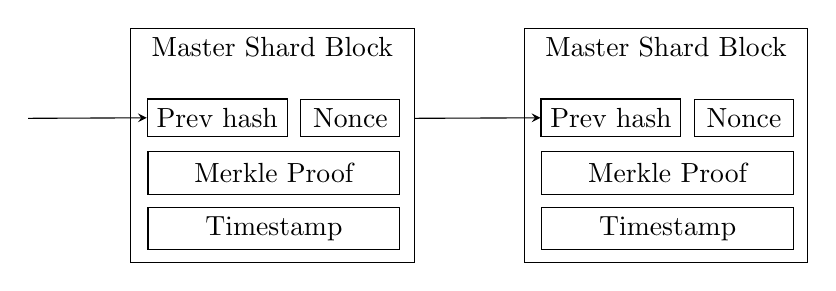
\begin{tikzpicture}
\centering
\node[draw,text depth = 2.5cm,minimum width=3.6cm,xshift=-1cm,yshift=-2em] at (-2.5, 1) (block1){Master Shard Block};
\node[draw] at ([yshift=1em,xshift=3.15em]block1.west)(prevhash1){Prev hash};
\node[draw,minimum width=1.26cm] at ([yshift=1em,xshift=7.96em]block1.west){Nonce};
\node[draw,minimum width=3.2cm, minimum height=0.54cm] at ([yshift=-1em,xshift=5.2em]block1.west){Merkle Proof};
\node[draw,minimum width=3.2cm] at ([yshift=-3em,xshift=5.2em]block1.west){Timestamp};

\node[draw,text depth = 2.5cm,minimum width=3.6cm,xshift=-1cm,yshift=-2em] at (2.5, 1) (block2){Master Shard Block};
\node[draw] at ([yshift=1em,xshift=3.15em]block2.west)(prevhash2){Prev hash};
\node[draw,minimum width=1.26cm] at ([yshift=1em,xshift=7.96em]block2.west){Nonce};
\node[draw,minimum width=3.2cm, minimum height=0.54cm] at ([yshift=-1em,xshift=5.2em]block2.west){Merkle Proof};
\node[draw,minimum width=3.2cm] at ([yshift=-3em,xshift=5.2em]block2.west){Timestamp};

\path[-stealth]
  (-1.7, 0.642) edge (prevhash2.west);
  
\path[-stealth]
  (-6.6, 0.642) edge (prevhash1.west);


\end{tikzpicture}
\end{center}

Using this design, the ratio of dishonest miners required to tamper with the ledger becomes $51/4 = 12.75\%$ while allowing asynchronous transaction processing. This is a great improvement but it is still not good enough to provide the same safety guarantees as Bitcoin does. We could use a single sector, however this would place greater strain on miners as they would have to validate 4 times the number of transactions before they emit a set of blocks. If we have 750kb blocks this would mean a miner has to validate $750kb \times 256 = 192mb$ of transaction data, hurting latency without providing concurrency to the system. With 4 sectors, we arrive at $750kb \times 64 = 48mb$ of transaction data which is written concurrently on each sector. Nodes listening to a single shard still require to process only 750kb of data. 

\section{Modified Green Proof-of-Work}
In order to further secure the system, we employ a modified variant of the Green Proof-of-Work model \cite{greenpow}. While also bringing the benefits of reducing the usual energy required for the mining process up to 50\%, we can leverage this model to artificially increase the hashpower required to tamper with a shard sector. In Green PoW, the mining process elapses in epochs, each consisting of two rounds. Each round represents a block appended to the chain. In the first round, all potential miners participate in finding a solution to the Proof-of-Work with the winner being elected to append the block in the first round. Then, all of the participants continue mining the same block until one or some of them find a solution. These miners are called runner-ups and are elected to mine the block in the second round. We can observe from this model that the hashpower required to append a second round block doubles as a potential attacker would have to mine the winning block from the first round along with the runnerup block. By using the same logic, we can increase the number of runnerup blocks required for a block to be mined in the second round from one to three. As such, we arrive at the same security properties as Bitcoin since we initially need 12.75\% of the hashpower to tamper with a sector and, by adjusting this parameter we increase the hashpower required to perform an attack to $12.75 \times 4 = 51\%$.

\section{Sequenced Proof-of-Work}
We further employ a Sequenced Proof-of-Work model in order to secure the network against tampering by powerful adversaries with access to vast resources such as state actors and centralised mining pools. There are two types of Proof-of-Work algorithms: ASIC resistant and ASIC friendly algorithms. Each has drawbacks in this regard, with the ASIC resistant algorithms exposing the network to hashpower marketplace attacks while the network is young but increasing its security if many retail miners are participating and ASIC resistant algorithms being vulnerable to centralised mining pools and state actors with vast resources but otherwise protecting the network as actors investing in dedicated hardware are less likely to attack the network due to the large upfront investment on their part. As such, we will use each type of algorithm in sequence for each mining epoch. We further sequence the ASIC mining epoch with a different, deterministically random ASIC friendly algorithm, thus requiring attackers to own the majority of hashpower by means of different hardware. The algorithm used in the next epoch is determined by using Consistent Hashing on the hash of the previous block. As such, it is impossible to predict the next ASIC friendly algorithm in the sequence.

While eventually, there will be an ASIC created for all ASIC friendly algorithms, sequencing ASIC friendly algorithms using some algorithms that are already used along with ones which are not widely used will protect the network while it is still young. This also creates incentives for miners with outdated ASICs built for other networks to reuse that hardware for the benefit of our network.

\section{State model}
In a sharded ledger, we have to think differently on how assets are controlled when compared to a single ledger. As we are following Bitcoin's model, each asset will be encoded as unspent outputs. As inter-shard transfers introduce great complexity to the system, they will not be possible. As such, fungible assets will be split equally across all shards. Purplecoins will be split equally by requiring each block to create a new coinbase output on a different shard in sequence. Another caveat is that in this model, one would often require to send a single transaction containing combined unspent outputs found on different shards. As such, these kind of transfers are by definition not atomic, and will partially settle at different times. Atomic transfers are possible only on single shards. 

Another problem is when new assets are encoded in the ledger, we need a way to safely partition them across all shards. Another problem arises in the case of non-fungible assets which could potentially be duplicated on different shards. 

\subsection{Asset specific accounts}
We further leverage and expand the transaction model of Bitcoin in order to solve these problems. An unspent output is encoded in Bitcoin as the amount of the output and the hash of the spending script of the output. The spender must provide this script when spending the output which contains their public key and signature along with any other spending rules. The hash of the spending script is the Bitcoin address owning that specific output. As such, we can encode asset specific rules by concatenating a second script hash to the address. Then, in order to spend, or issue a specific asset both the asset script and spending script have to perfectly match the address. As each asset has a strongly differentiated type of address, they cannot be duplicated across shards as it would yield a different address half. We can then encode rules in the asset script such as:
\begin{enumerate}
  \item Asset x can only be created on a subset of shards or a single shard.
  \item Asset y can only be issued if a signature is provided by a specific public key.
  \item Asset z can only be spent if a signature is also provided by the issuer. 
\end{enumerate}

We can further employ Merkelised Abstract Syntax Trees \cite{mast} to allow different sets of conditions to be used inter-changeably on a specific asset.

\clearpage

\section{Conclusion}
We have proposed a tamper-proof electronic ledger system with advanced scalability and transactional properties. We have started by following Bitcoin's model and expanded upon it by allowing stateless transaction validation and employing secure sharding at the state layer in order to increase the transaction throughput of the system. The result is a fundamentally scalable system, that can be reasonably dealt with by node operators, without additional storage and bandwidth costs and can even run by only relying on RAM, allowing its implementation in a similar manner as how a telephone grid is built. 

\begin{thebibliography}{9}

\bibitem{btc}
Bitcoin: A Peer-to-Peer Electronic Cash System.
Satoshi Nakamoto. \textit{
https://bitcoin.org/bitcoin.pdf
}

\bibitem{merkle}
A Digital Signature Based on a Conventional Encryption Function.
Ralph C. Merkle.
Elxsi 2334 Lundy Place San Jose, CA 95131.
https://people.eecs.berkeley.edu/~raluca/cs261-f15/readings/merkle.pdf

\bibitem{ca}
An Overview of Cryptographic Accumulators.
Ilker Ozcelik$^1$$^,$$^2$, Sai Medury$^1$, Justin Broaddus$^1$, Anthony Skjellum$^1$. \\
$^1$ SimCenter \& Department of Computer Science and Engineering, University of Tennessee at Chattanooga, Chattanooga, Tennessee, USA. \\$^2$ Recep Tayyip Erdogan, Rize, Turkey\textit{
https://arxiv.org/pdf/2103.04330v1.pdf
}

\bibitem{greenpow}
Green-PoW: An energy-efficient blockchain Proof-of-Work consensus algorithm.
Noureddine Lasla, Member, IEEE, Lina Salim Alsahan, Mohamed Abdallah, Senior Member, IEEE
and Mohamed Younis, Senior Member, IEEE.
\textit{
https://arxiv.org/pdf/2007.04086.pdf
}

\bibitem{mast}
Merkelised Abstract Syntax Trees.
Jeremy Rubin, Manali Naik, Nitya Subramanian.
https://www.mit.edu/$\sim$jlrubin/public/pdfs/858report.pdf

\end{thebibliography}
\end{document}